\documentstyle[info-utf8,graphicx]{jarticle}
%
% 著者の所属が1つの研究機関の場合の様式
%
%\author{情報太郎\Email{hokkaido@ipsj.or.jp}
%\hspace{5mm}情報次郎
%\hspace{5mm}情報三郎 \\
%(北大情報科学)\contactto{札幌市北区北14条西9丁目北海道大学大学院情報科学研究科}}
%
% 著者が複数の研究機関に所属する場合の様式
%
\author{%
\begin{tabular}{ccc}
武信雄平\Email{\,\,\,b1016127@fun.ac.jp} &
奥野拓 \\
\multicolumn{2}{c}{%
(公立はこだて未来大学)\contactto{\,\,\,北海道函館市亀田中野町116番地2 公立はこだて未来大学システム情報科学部}}
\end{tabular}}

\title{観光スポットと移動経路に対する嗜好を考慮した \\
観光ルート推薦システムの構築}

\begin{document}
\maketitle

\section{はじめに}\label{sec:はじめに}
土地勘のない観光客にとって,観光を快適に楽しむためには,事前に観光プランを作成することが重要である.
そのため,WebサイトやSNSなどを利用し,観光に必要な情報の収集や移動手段などを考慮したスケジュールの作成が必要となる.
しかし,WebサイトやSNSなどから観光に必要な情報を見つけることや,移動手段などを考慮してスケジュールを作成することは,観光客にとって負担が大きい.
そのため,観光客の負担が少ない観光プラン作成支援システムが必要である.
個々の観光客に合った観光プランを作成するためには,観光スポットや移動経路に対する嗜好を考慮した観光ルートを作成する必要がある.


本研究では,観光客の観光スポットと移動経路に対する嗜好を考慮した観光プランの作成を支援する.
そのために,個々の観光客に合った満足度が高い観光ルートを生成することを目指す.

\section{観光ルートの自動生成に関する研究}\label{sec:観光ルートの自動生成に関する研究}
ユーザの観光スポットに対する嗜好を基にした観光ルートの自動生成と,対話的なルート変更が可能なCT-Planner3がある\cite{倉田}.
CT-Planner3では,ユーザがレーダーチャートを操作することにより,自らの嗜好を直接入力する.
さらに,観光したい,もしくはしたくない観光スポットをユーザが設定できる.
しかし,移動経路に対する嗜好は考慮されていない.
移動経路に対する嗜好とは,観光や移動にかける時間,費用などをどの程度重視するかのことである.


他に,ユーザの嗜好と消費するリソースを考慮した複数の観光ルートを提示することで,ユーザの観光ルート決定を支援する研究がある\cite{平野}.
この研究では,まずユーザが消費するリソースとして,金銭,時間,スタミナの3つと観光によって得られる満足度のトレードオフを考慮し,パレート最適解となる観光ルートを生成する.
その後,生成した観光ルートを複数提示し,ユーザがその中からルートを選択する.
しかし,ユーザが各要因をどの程度重視するかを調整できないため,観光スポットと移動経路に対するユーザの嗜好に合ったルートが生成されにくい.

\section{観光ルートの自動生成システム}\label{sec:観光ルート自動生成システム}
本研究では,観光スポットと移動経路に対するユーザの嗜好に合った観光ルートを自動生成できるシステムを構築する.
% システムのイメージをFig.\ref{fig:観光ルートを表示する画面}に示す.
構築するシステムでは,始めにユーザに出発地点,終着地点,出発時刻,終着時刻を入力してもらう.
それらの入力後,どのような観光スポットや移動経路を好むかを各特徴のスライダーを用いて入力してもらう(Fig.\ref{fig:ユーザの嗜好を入力する画面}).
各特徴とは,「自然」や「文化」などの観光スポットの嗜好に関する項目や「移動費」や「移動時間」などの移動経路の嗜好に関する項目のことである.
その後,ユーザの入力内容を基に,ルートを自動で生成する.
ルートの生成方法については,\ref{sec:観光ルート自動生成アルゴリズム}章にて記述する.
その後,生成されたルートから特徴が異なるいくつかのルートを表示する.
その中から1つを選択すると,地図上に移動経路と観光スポットの位置を表示する.
また,そのルートの特徴と,どのようなスケジュールで観光スポットを回るかも表示する.
その際地図上では,移動経路と観光スポットの位置を表示する.
また,表示されている観光スポット名を選択すると,地図部分の代わりに,選択された観光スポットの情報として,その場所の説明文や営業時間などを表示する.
表示されたルートのいずれかをユーザが気に入った場合は,そのルートのスケジュール下部にある「このルートにする」を選択してもらう.
表示されたルートとは異なる特徴を持つルートを知りたい場合は,「別の特徴を持つルートを表示する」を選択してもらう.
表示されているルートを改善したルートを知りたい場合,改善したいルートのスケジュール下部にある「このルートの一部を改善したルートを新たに作成する」ボタンを選択してもらう.
その後,改善したい部分をチェックボックスを用いて選択してもらう(Fig.\ref{fig:ルートの改善部分を選択する画面}).
改善できる部分は,そのルート内の訪問したくない観光スポットを選択する,観光スポットや移動経路に関する各項目をよりユーザの好みに近づくように調整する,の2つである.
その後,それに合わせたルートの生成を再度行う.
% 生成されたルートは再度Fig.\ref{fig:観光ルートを表示する画面}のように表示する.
生成されたルートから再度特徴が異なるいくつかのルートを表示する.
これらをユーザが気に入ったコースが表示されるまで繰り返す.
% \begin{figure}[h]
%   \begin{center}
%   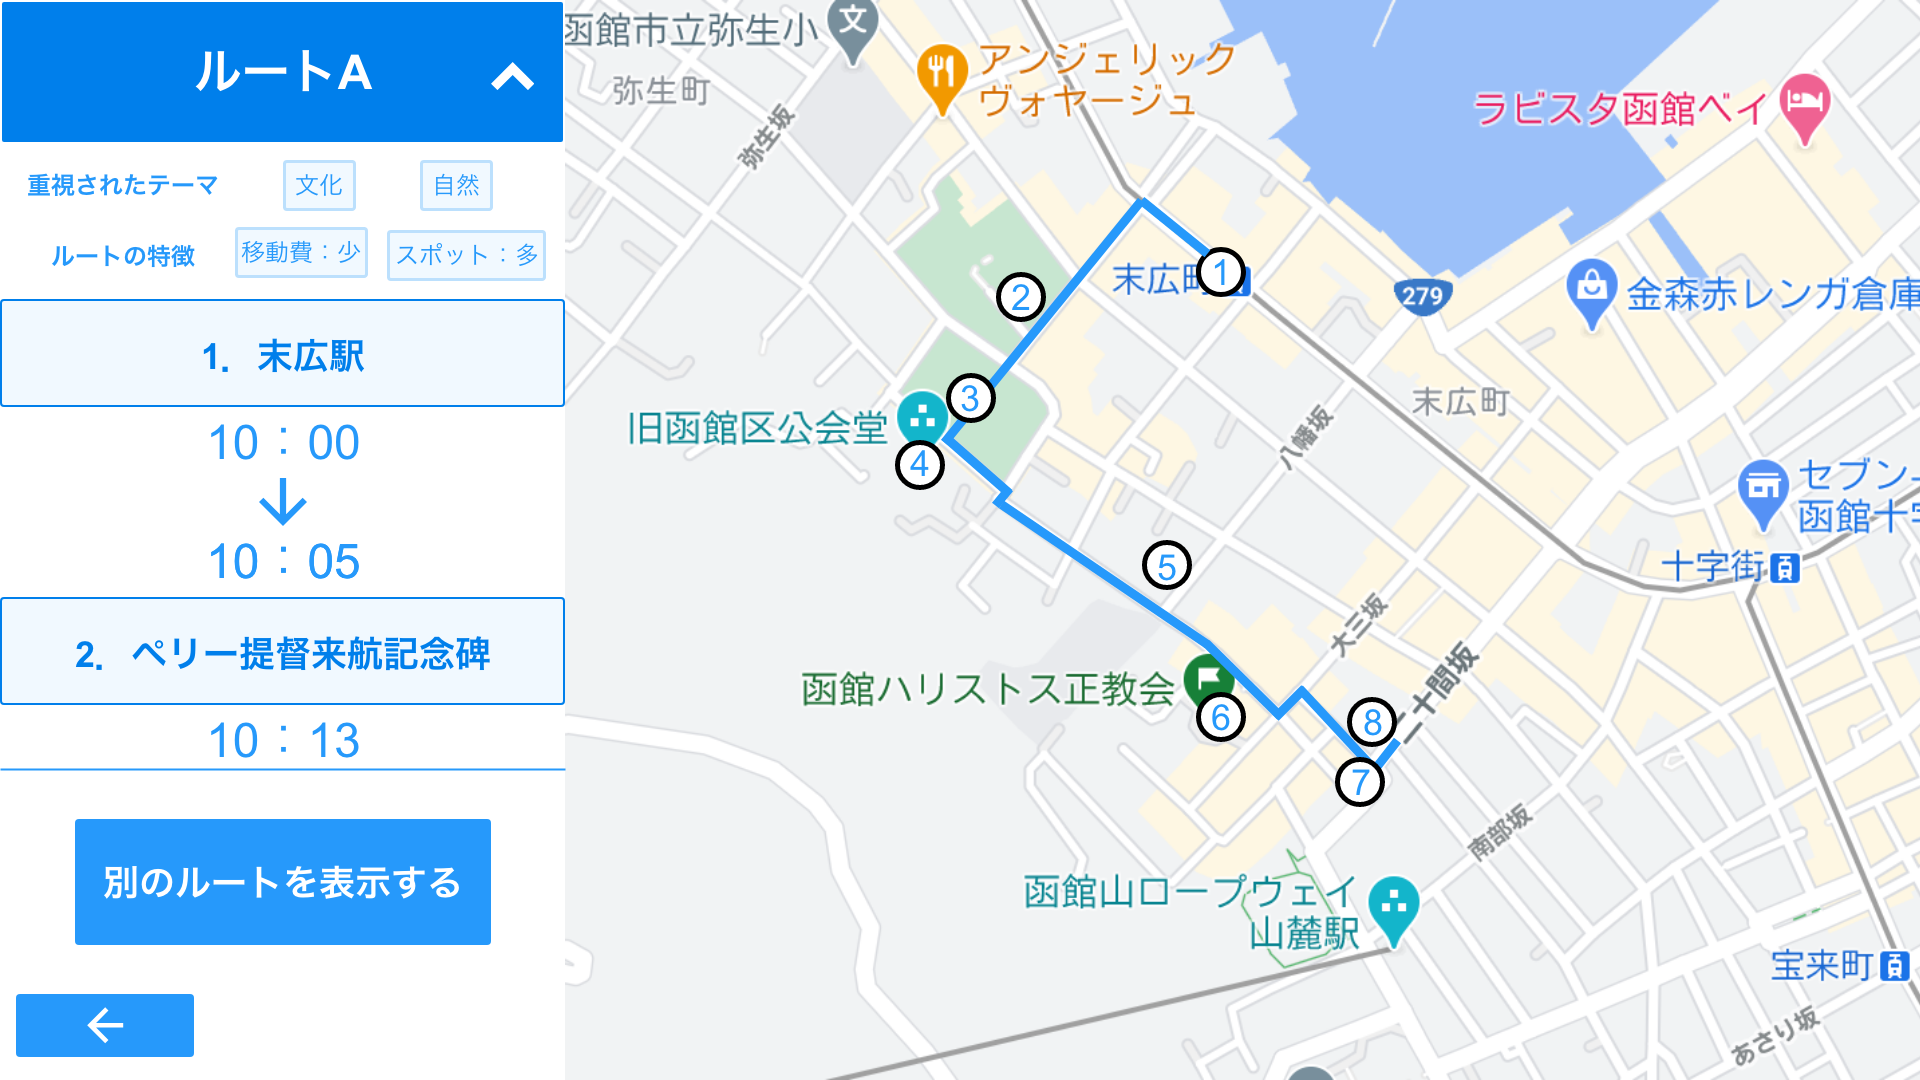
\includegraphics[width=8.5cm,bb=0 0 1980 1080]{sysimage1.png}
%   \end{center}
%   \caption{観光ルートを表示する画面} 
%   \label{fig:観光ルートを表示する画面}
% \end{figure}

\begin{figure}[h]
  \begin{center}
  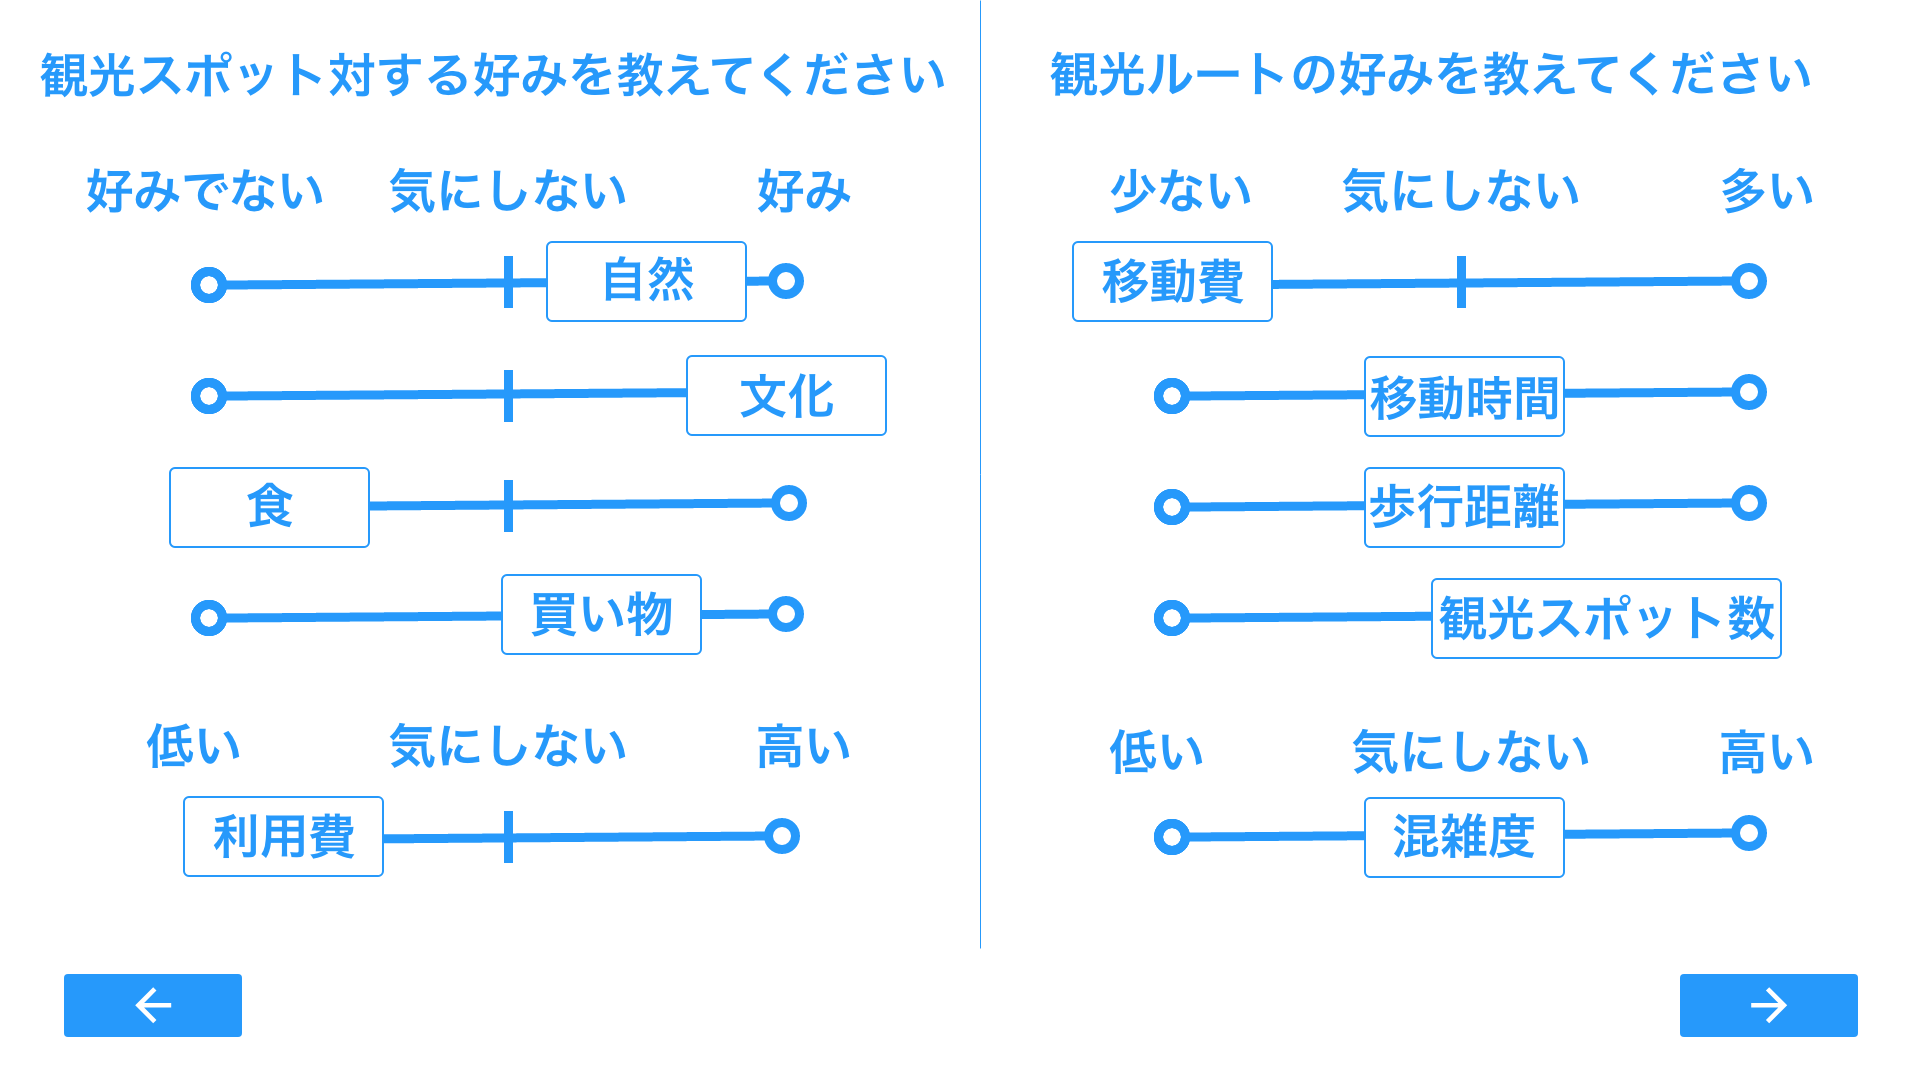
\includegraphics[width=8.5cm,bb=0 0 1980 1080]{sysimage2.png}
  \end{center}
  \caption{ユーザの嗜好を入力する画面} 
  \label{fig:ユーザの嗜好を入力する画面}
\end{figure}

\begin{figure}[h]
  \begin{center}
  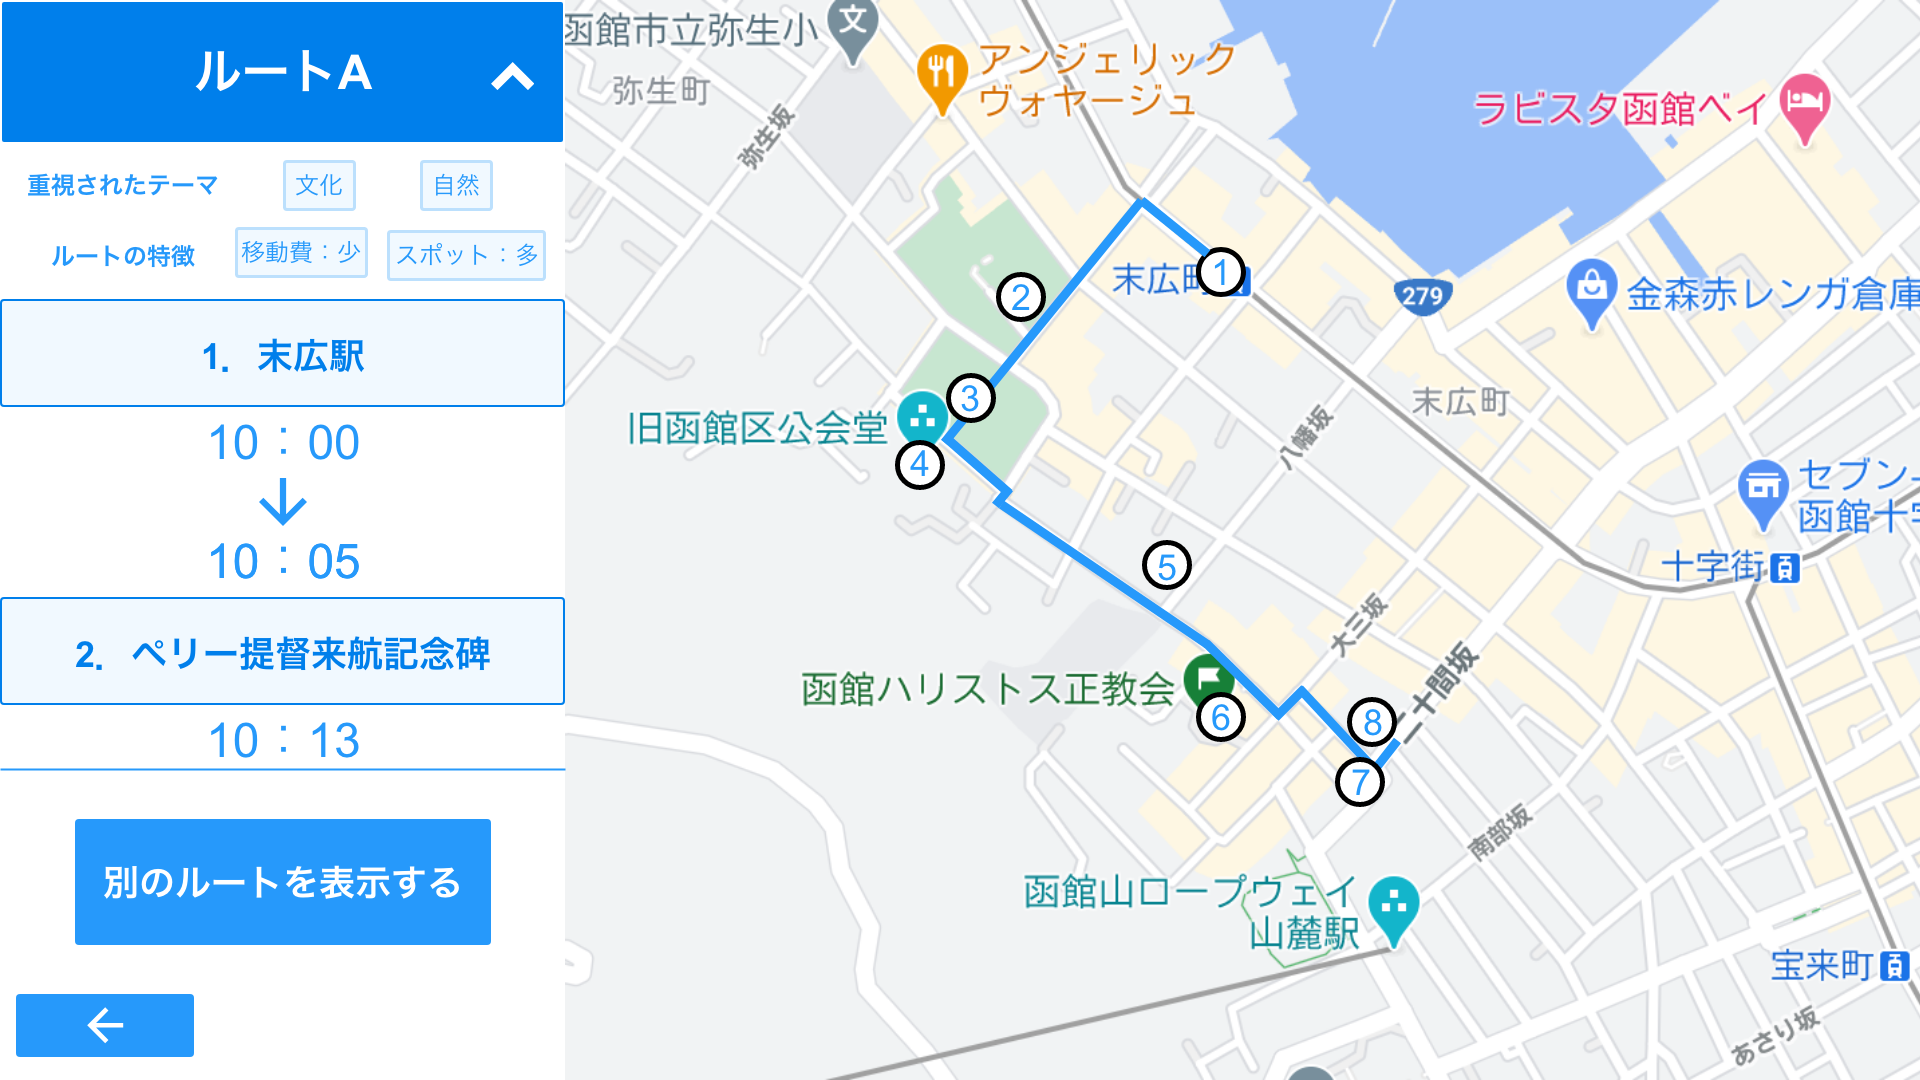
\includegraphics[width=8.5cm,bb=0 0 1980 1080]{sysimage1.png}
  \end{center}
  \caption{ルートの改善部分を選択する画面(図は未修正)} 
  \label{fig:ルートの改善部分を選択する画面}
\end{figure}

\section{観光ルートの自動生成アルゴリズム}\label{sec:観光ルート自動生成アルゴリズム}
本研究では,観光スポットと移動経路に対するユーザの嗜好を反映したルートの自動生成を行う.
そのために,Debらが提案した多目的遺伝的アルゴリズムであるNSGA-I\hspace{-.1em}I\hspace{-.1em}I\cite{NSGA3}とそれらの手法の解に対して任意の特徴を改善できる岸上らの研究\cite{岸上}を基にアルゴリズムを作成する.
多目的最適化に遺伝的アルゴリズムを用いた場合,目的の数が増加するほど解が収束しにくくなるという問題がある.
NSGA-I\hspace{-.1em}I\hspace{-.1em}Iではそれを解決するために,reference pointの概念を導入することにより,ユーザが探索を進めたい嗜好方向に対して解を収束させることができる.
以下に本研究におけるアルゴリズムの特徴的な部分を記述する.
\subsection{初期個体の作成}\label{sec:初期解の作成}
まず初めに,観光スポット全体からランダムに観光スポットを選択し,それらを最短経路で結ぶ.
その際,ユーザの嗜好に合った観光スポットが選ばれやすいようにする.
また,初期個体を作成する段階で最短経路を求めることにより,初期個体が優秀になりやすくなる.
これらを初期個体数の数だけ行う.
\subsection{交叉}\label{sec:交叉}
交叉には一点交叉を用いる.
また,解を選択する際に,reference pointとPBI距離を用いる.
reference pointは事前に設定されており,探索空間を均一に分割するように設定する.
それ以外に,ユーザの嗜好に合わせたreference pointも追加で設定する.
その後,全ての解を嗜好の方向性に応じてreference pointに関連づけする.
PBI距離はその解の優秀さを示しており,観光スポットや移動経路の嗜好を満たすほど大きくなり,関連づけされた嗜好の方向性から離れているほど小さくなる.
これらを用いることで,様々な嗜好の方向性を持つ優秀な解同士を交叉することができる.
それに加えて本研究では,交叉する地点の最短経路の長さも用いる.
それにより,交叉する親個体同士の相性も考慮でき,より優秀な解が生まれやすくなる.
\subsection{変異}\label{sec:変異}
変異の方法は\ref{sec:観光ルートの自動生成に関する研究}章で紹介した平野らの研究\cite{平野}と同様に,増加変異と減少変異のどちらかをランダムに行う.
\subsection{淘汰}\label{sec:淘汰}
初期個体,交叉した個体,突然変異した個体からより優秀な個体を次世代に残す.
そのために,各reference pointに関連づけされた個体から同数の個体が選択されるようにする.
その際,PBI距離が最も大きな個体から順に選択する.
これにより,多様性のある個体を次世代に残すことができる.
\subsection{ユーザによる解の評価}\label{sec:ユーザによる解の評価}
reference pointをランダムにいくつか選択し,それぞれに関連する個体の中で最も優秀な個体を表示する.
その後,「このルートの一部を改善したルートを新たに作成する」が選択された場合,\cite{岸上}の原点を移動させる方法を用いて,一部の特徴を改善した解を生成するために,追加で\ref{sec:交叉}節から\ref{sec:淘汰}節を繰り返し行う.
その後,reference pointをランダムいくつか選択し,それぞれに関連する個体の中で最も優秀な個体を再度表示する.
これをユーザが満足するまで行う.

\section{アルゴリズムの評価}\label{sec:アルゴリズムの評価}
\ref{sec:観光ルート自動生成アルゴリズム}章のアルゴリズムを用いて,観光ルート推薦システムを構築し,有用性を検証するために評価実験を行う.
評価方法として,被験者を半数に分け,片方がWebサイトやSNSなどを用いて観光ルートを作成した後に,提案手法で観光ルートを作成する.
もう片方は逆の順番で観光ルートを作成する.
その後,被験者にどちらの観光ルートを利用したいかアンケートを実施する.
さらに,抽出した嗜好の中で,ユーザが重要視した評価項目に着目した定性的な比較評価も行う予定である.

\section{まとめ}\label{sec:まとめ}
本研究では,多目的遺伝的アルゴリズムであるNSGA-I\hspace{-.1em}I\hspace{-.1em}Iを用いて,観光スポットと移動経路に対するユーザの嗜好を反映したルートの自動生成とその評価方法について説明した.
今後は\ref{sec:観光ルート自動生成アルゴリズム}章で述べたアルゴリズムを実装し,評価実験を行う.
その後,評価実験の結果を基にアルゴリズムの改善を行う.

\begin{thebibliography}{99}
\bibitem{倉田} 倉田陽平:CT-Planer 3:Web上での対話的な旅行プラン作成支援,観光科学研究,5,pp.159-165(2012)
\bibitem{平野} 平野陽大,諏訪博彦,安本慶一:ユーザのリソース消費を考慮した意思決定支援のための複数観光経路提示手法,情報処理学会,マルチメディア,分散協調とモバイルシンポジウム2019論文集,pp.830-839(2019)
\bibitem{NSGA3} K. Deb,H. Jain:An evolutionary many-objective optimization algorithm using reference-point-based nondominated sorting approach, part I: Solving problems with box constraints,IEEE Transactions on Evolutionary Computation,Vol.18,pp.577-601(2014)
\bibitem{岸上} 岸上利裕,吉川大弘:reference lineに基づくユーザの嗜好方向探索手法の提案,進化計算学会論文誌,Vol.6,pp.31-41(2015)
\end{thebibliography}
\end{document}
%
%
% End of file: sample.tex
